\documentclass[11pt]{article}
\usepackage[margin=1in]{geometry}
\usepackage{amsmath,amssymb,amsthm,mathtools,bbm}
\usepackage{enumitem}
\usepackage{hyperref}
\usepackage{thmtools}
\usepackage{bm}
\usepackage{booktabs}

\hypersetup{
  colorlinks=true,
  linkcolor=blue,
  citecolor=blue,
  urlcolor=blue
}

\declaretheorem[name=Theorem,numberwithin=section]{theorem}
\declaretheorem[name=Proposition,sibling=theorem]{proposition}
\declaretheorem[name=Lemma,sibling=theorem]{lemma}
\declaretheorem[name=Corollary,sibling=theorem]{corollary}
\declaretheorem[name=Definition,style=definition,numberwithin=section]{definition}
\declaretheorem[name=Remark,style=remark,sibling=theorem]{remark}

\newcommand{\X}{\mathcal{X}}
\newcommand{\Y}{\mathcal{Y}}
\newcommand{\Z}{\mathcal{Z}}
\newcommand{\N}{\mathbb{N}}
\newcommand{\E}{\mathbb{E}}
\newcommand{\1}{\mathbbm{1}}
\newcommand{\KL}{\mathrm{D}}
\newcommand{\bits}{\;\mathrm{bits}}
\newcommand{\nats}{\;\mathrm{nats}}
\newcommand{\law}{\mathcal{L}}
\newcommand{\code}{\mathcal{E}}
\newcommand{\codelen}{\mathsf{L}}
\newcommand{\push}{\#}
\newcommand{\RR}{\mathbb{R}}

\title{Evidence Holonomy and Entropy Production:\\
From Universal Coding to Irreversibility}
\author{Joshua Winters\\Independent Researcher\\\texttt{josh@friendmachine.co}}
\date{August 27, 2025}

\begin{document}
\maketitle

\begin{abstract}
We define an ``evidence holonomy'' functional on loops of representation transforms applied to sample paths. Using pointwise universality of code lengths for stationary ergodic processes, we prove two reductions: (i) \textbf{representation-space holonomy} converges (up to $o(n)$) to the entropy-rate difference $h(Q)-h(P)$; (ii) \textbf{KL-holonomy}—implemented by transporting a universal code trained under $P$ to one trained under $Q$—converges to the relative-entropy rate $\mathsf{d}(P\|Q)$. For finite-state Markov processes, KL-holonomy along the time-reversal loop equals the entropy-production rate $\sigma$ (bits/step). We show asymptotic code-invariance of KL-holonomy and validate the framework on Arrow-of-Time benchmarks (audio, sensors, finance).
\end{abstract}

\section{Setup and Definitions}

\paragraph{Alphabet and path space.} Fix a finite alphabet $\X$. Let $\X^n$ denote length-$n$ strings and $\X^{\N}$ the one-sided sequence space with its product $\sigma$-algebra. Let $P$ be a stationary ergodic probability measure on $(\X^{\N},\mathcal{F})$. Write $X_{0:n-1}$ for the length-$n$ prefix of a sample from $P$ and $P_n$ for its law on $\X^n$.

\paragraph{Universal codes.}
A \emph{universal code} on alphabet $\mathcal{A}$ is a map $\code_{\mathcal{A}}:\bigcup_{n\ge 1}\mathcal{A}^n\to \RR_+$ assigning a code length in bits to any finite string, such that for every stationary ergodic law $Q$ on $\mathcal{A}^{\N}$,
\begin{equation}\label{eq:universality}
\frac{1}{n}\Big(\code_{\mathcal{A}}(Y_{0:n-1}) + \log_2 Q_n(Y_{0:n-1})\Big) \xrightarrow[n\to\infty]{Q\text{-a.s.}} 0,
\end{equation}
with convergence also in $L^1(Q)$. Classical examples include LZ78, Krichevsky--Trofimov mixtures for finite-order Markov models, and CTW \cite{ziv1978,kt1981,willems1995ctw,shields1996,csiszarshields2004}.

\paragraph{Standing assumptions.}
Unless stated otherwise, alphabets are finite; processes are stationary and ergodic;
and when KL rates are finite we assume absolute continuity $P\ll Q$.
All identities are per-symbol, up to $O(1)$ boundary terms (negligible when divided by $n$).
All logs are base 2.

\paragraph{Representation transforms and loops.}
For each $n$, let $F_{i,n}$ be a measurable map
$F_{i,n}:\X_{i-1}^{\,n_{i-1}(n)}\to\X_i^{\,n_i(n)}$, where the alphabets
$\X_i$ may differ by step, and $n_0(n)=n$. Define successive images
$x^{(0)}=x\in\X^n$ and $x^{(i)} = F_{i,n}\circ\cdots\circ F_{1,n}(x^{(0)}) \in \X_i^{\,n_i(n)}$.
A finite list $\gamma=(F_{1,n},\ldots,F_{m,n})$ is a \emph{loop at scale $n$}
if $\X_m=\X_0=\X$ and $n_m(n)=n+O(1)$. We write $L_n=F_{m,n}\circ\cdots\circ F_{1,n}$.
When $n_m(n)\neq n$, evaluations are aligned by truncating/offsetting one argument
(e.g., ``tail alignment'' $X_{1:n-1}$ versus a length $n\!-\!1$ loop output);
this contributes only $O(1)$ boundary terms, negligible after dividing by $n$.

\paragraph{Why `holonomy'?}
In differential geometry, holonomy measures the failure of a vector to return unchanged after
parallel transport around a closed loop; the effect depends on the connection and reflects curvature.
Here, the `vector' is a description length (or log-likelihood) assigned by an observer (a code),
the `connection' is the rule transporting this observer along a loop of representation transforms,
and the holonomy is the net change after completing the loop.
Zero holonomy corresponds to flatness (e.g., bijective relabelings), whereas coarse-grainings or
time-reversal in nonequilibrium systems induce positive `curvature' detected by nonzero holonomy.
This analogy motivates the terminology and clarifies why observer choice acts like a gauge: our
KL-holonomy rate is asymptotically gauge-invariant across universal codes.

\subsection{Two holonomy functionals}

\begin{definition}[Representation-space holonomy]\label{def:holonomy-out}
Given universal codes $\code_{\X_i}$ for intermediate alphabets, define
\begin{align*}
\mathrm{Hol}_{n}^{\mathrm{out},\gamma}(x)
  &= \sum_{i=1}^m \Big(\code_{\X_i}\big(x^{(i)}\big)-\code_{\X_{i-1}}\big(x^{(i-1)}\big)\Big)\\
  &= \code_{\X}\big(L_n(x)\big)-\code_{\X}(x).
\end{align*}
\end{definition}

\begin{definition}[KL (observer-transported) holonomy]\label{def:holonomy-kl}
Let $P_n$ be the law of $X_{0:n-1}$ and $Q_n=(L_n)\# P_n$. Define the ideal codelengths
$\mathcal{L}^{(P)}_n(x)=-\log_2 P_n(x)$ and $\mathcal{L}^{(Q)}_n(x)=-\log_2 Q_n(x)$.
The (ideal) KL holonomy is
\[
\mathrm{Hol}^{\mathrm{KL},\gamma}_n(x) \;=\; \mathcal{L}^{(Q)}_n(x) - \mathcal{L}^{(P)}_n(x)
\;=\; \log_2 \frac{P_n(x)}{Q_n(x)}.
\]
Hence $\tfrac{1}{n}\E_P[\mathrm{Hol}^{\mathrm{KL},\gamma}_n] = \tfrac{1}{n}\KL(P_n\|Q_n) \to \mathsf{d}(P\|Q)$.
\emph{Implementation note.} In experiments we approximate $\mathcal{L}^{(P)}_n$ and $\mathcal{L}^{(Q)}_n$
with universal coders; under standard log-loss consistency for the model class used, the empirical
rates converge in $L^1$ to the ideal ones.
\end{definition}

\section{Reductions via Universality}

\noindent\emph{Convention.} All statements below are per symbol, with $O(1)$
boundary discrepancies (e.g., from alignment) absorbed into the $o(1)$ terms.

\begin{lemma}[Pointwise reductions]\label{lem:pointwise}
Assume \eqref{eq:universality} for the relevant laws.
\begin{enumerate}[leftmargin=2em,itemsep=0.25em]
\item For $\mathrm{Hol}^{\mathrm{out}}$: with $\code_\X$ universal for both $P$ and the pushforward process,
\begin{equation}\label{eq:hol-out-reduction}
\frac{1}{n}\Big(\mathrm{Hol}_{n}^{\mathrm{out},\gamma}(X_{0:n-1}) - \log_2\frac{P_n(X_{0:n-1})}{Q_n(L_n(X_{0:n-1}))}\Big) \xrightarrow[n\to\infty]{P\text{-a.s.}} 0.
\end{equation}
\item For $\mathrm{Hol}^{\mathrm{KL},\gamma}$:
\begin{equation}\label{eq:hol-kl-reduction}
\frac{1}{n}\Big(\mathrm{Hol}_{n}^{\mathrm{KL},\gamma}(X_{0:n-1}) - \log_2\frac{P_n(X_{0:n-1})}{Q_n(X_{0:n-1})}\Big) \xrightarrow[n\to\infty]{P\text{-a.s.}} 0.
\end{equation}
\end{enumerate}
Both convergences also hold in $L^1(P)$.
\end{lemma}
\begin{proof}
Apply \eqref{eq:universality} (Barron's strong pointwise coding theorem) to each code/law pair and subtract the limits; see \cite{barron1985,csiszarshields2004,shields1996}.
\end{proof}

Averaging yields the two central identities.

\begin{theorem}[Expectation-level reductions]\label{thm:exp_reductions}
Under $L^1$ universality,
\begin{align}
\frac{1}{n}\,\E_P\big[\mathrm{Hol}_{n}^{\mathrm{out},\gamma}\big]
&= h(Q)-h(P)+o(1), \label{eq:exp-out}\\[0.35em]
\frac{1}{n}\,\E_P\big[\mathrm{Hol}_{n}^{\mathrm{KL},\gamma}\big]
&= \frac{1}{n}\,\KL(P_n\|Q_n)\;\xrightarrow[n\to\infty]{}\; \mathsf{d}(P\|Q)\;\ge 0. \label{eq:exp-kl}
\end{align}
\end{theorem}
\begin{proof}
Take expectations in \eqref{eq:hol-out-reduction}--\eqref{eq:hol-kl-reduction} and note
$\E_P[-\log_2 P_n(X_{0:n-1})]=H(P_n)$, $\E_P[-\log_2 Q_n(L_n(X_{0:n-1}))]=H(Q_n)$, and $\E_P\big[\log_2 \tfrac{P_n(X)}{Q_n(X)}\big]=\KL(P_n\|Q_n)$.
\end{proof}

\begin{remark}[Scope]
Equation~\eqref{eq:exp-out} is gauge-invariant and measures net compression or expansion under the loop. Equation~\eqref{eq:exp-kl} is the \emph{irreversibility} functional implemented in our code (KL-rate holonomy): it is observer-transported and non-negative.
\end{remark}

\section{Canonical Loops and Corollaries}

\subsection{Gauge invariance for bijective loops}

\begin{corollary}[Gauge invariance]\label{cor:gauge}
If each $F_{i,n}$ is a bijection and the loop is the identity on $\X^n$, then
\[
\frac{1}{n}\,\mathrm{Hol}_{n}^{\mathrm{out},\gamma}(X_{0:n-1}) \to 0
\quad\text{and}\quad
\frac{1}{n}\,\mathrm{Hol}_{n}^{\mathrm{KL},\gamma}(X_{0:n-1}) \to 0
\]
in $P$-probability and in $L^1(P)$.
\end{corollary}
\begin{proof}
Then $Q_n=P_n$ for all $n$, so both \eqref{eq:exp-out} and \eqref{eq:exp-kl} vanish.
\end{proof}

\subsection{Coarse-graining loops via channels}
Let $K_n$ be a (possibly many-to-one) Markov kernel on $\X^n$ and $R_n$ any measurable right-inverse (a ``lift'') so that $L_n:=R_n\circ K_n:\X^n\to\X^n$ is a loop. If $Q_n:=L_n\push P_n$ arises from a stationary $Q$, then \eqref{eq:exp-kl} gives
\[
\frac{1}{n}\,\E_P\big[\mathrm{Hol}_{n}^{\mathrm{KL},\gamma}\big] \to \mathsf{d}(P\|Q) \ge 0,
\]
i.e.\ KL holonomy is non-negative by construction (by non-negativity of KL).
Moreover, if both $P_n$ and $Q_n$ are mapped through the same observation channel,
data processing yields a lower bound on the holonomy of the observed records.

\paragraph{When is the pushforward stationary?}
For a general sequence of maps $L_n$, the marginals $Q_n=(L_n)\#P_n$ need not be the $n$-marginals of any stationary process.
A sufficient condition is that the loop arises from a shift-commuting, finite-memory map on the two-sided shift
(a sliding-block code): i.e., there exist $F$ and memory $m$ such that $(L_n(x))_t = F(x_{t-m:t+m})$ for all $t$,
and $F$ commutes with the left-shift.
Then, if $P$ is stationary, so is the pushforward process $Q$. The canonical time-reversal loop and
coarse-graining channels satisfy this property. In our theorems that invoke entropy-rate limits for $Q$,
we implicitly assume such a stationary extension exists (or restrict to cases where it is direct, e.g. time reversal).

\subsection{Time reversal and entropy production for Markov chains}

Let $P$ be a stationary Markov chain on $\X=\{1,\dots,k\}$ with transition $T$ and stationary $\pi$. Its time-reversal $P^{\mathrm{rev}}$ has transitions $T^\ast_{ji}=\frac{\pi_i T_{ij}}{\pi_j}$. 

\paragraph{Canonical time-reversal loop.}
Let $x_{0:n-1}$ be a path from a stationary finite-state Markov chain $P$ with transition matrix $T$.
Define three maps on paths of length $n$:
(i) the transition encoder $E$ mapping $(x_{t-1},x_t)_{t=1}^{n-1}$ to the edge sequence;
(ii) reversal $R$ mapping an edge sequence $(e_1,\dots,e_{n-1})$ to $(e_{n-1},\dots,e_1)$;
(iii) a state decoder $D$ that reconstructs a path from the reversed edge sequence given the terminal
state $x_{n-1}$ as anchor.
The loop is $L_n := D \circ R \circ E$. One checks that $(L_n)\# P_n = P_n^{\mathrm{rev}}$,
the $n$-path law of the time-reversed chain.

\begin{quote}
\textbf{Algorithm:} Time-reversal loop $L_n$\\
\textbf{Input:} $x_{0:n-1}$\\
1. $E \leftarrow ((x_{t-1},x_t))_{t=1}^{n-1}$\\
2. $E' \leftarrow \mathrm{reverse}(E)$\\
3. $\hat{x}_{n-1} \leftarrow x_{n-1}$ \quad (anchor)\\
4. For $t=n-1$ down to $1$:\\
\quad Set $\hat{x}_{t-1}$ as the unique predecessor such that $(\hat{x}_{t-1},\hat{x}_{t})=E'_{n-t}$\\
\textbf{Output:} $L_n(x)=\hat{x}_{0:n-1}$
\end{quote}

\begin{remark}[Practical variant]
Our implementation uses a length-$n\!-\!1$ variant:
encode transitions, reverse, and \emph{decode the second state} of each reversed
edge. We then evaluate on $X_{1:n-1}$ to match lengths. This avoids explicit
anchoring by $x_{n-1}$ and differs only by $O(1)$ boundary terms, hence the
per-symbol limits are unchanged.
\end{remark}

\begin{theorem}[KL holonomy rate equals entropy production]\label{thm:EP}
For the Markov setting above,
\begin{equation}\label{eq:EP_rate}
\mathsf{d}(P\|P^{\mathrm{rev}}) \;=\; \sum_{i,j}\pi_i T_{ij}\,\log_2\frac{\pi_i T_{ij}}{\pi_j T_{ji}} \;=\; \sigma\quad(\text{bits/step}),
\end{equation}
and the KL-holonomy satisfies
\begin{equation}\label{eq:EP_hol}
\frac{1}{n}\,\E_P\big[\mathrm{Hol}_{n}^{\mathrm{KL},\mathrm{time\text{-}rev}}\big] \;\to\; \sigma.
\end{equation}
\end{theorem}
\begin{proof}
The path log-likelihood ratio between $P$ and the reversed path law under $P^{\mathrm{rev}}$ is
\[
\log\frac{P_n(X_{0:n-1})}{P_n^{\mathrm{rev}}(R_n(X_{0:n-1}))}
= \sum_{t=1}^{n-1}\log\frac{\pi_{X_t}}{\pi_{X_{t-1}}}
+ \sum_{t=1}^{n-1}\log\frac{T_{X_{t-1}X_t}}{T_{X_t X_{t-1}}}.
\]
The stationary term telescopes to $O(1)$; divide by $n$ and take expectations. Identity \eqref{eq:EP_rate} is standard in stochastic thermodynamics \cite{schnakenberg1976,seifert2012}. Equation \eqref{eq:EP_hol} is \eqref{eq:exp-kl} with $Q=P^{\mathrm{rev}}$.
\end{proof}

\begin{remark}[Absolute continuity]
The rate in \eqref{eq:EP_rate} is finite iff $T_{ij}>0 \Rightarrow T_{ji}>0$
for all $i,j$; otherwise $\mathsf{d}(P\|P^{\mathrm{rev}})=+\infty$.
\end{remark}

\begin{remark}[Why not merely $h(Q)-h(P)$?]
For stationary Markov chains, $h(P)=h(P^{\mathrm{rev}})$, so representation-space holonomy would vanish. The KL version (observer-transported) returns the irreversible production $\sigma$.
\end{remark}

\subsection{General ergodic reversal}
Let $P^\ast$ be any stationary time-reversed process absolutely continuous w.r.t.\ $P$ on cylinders, with finite $\mathsf{d}(P\|P^\ast)$. Then, by the same argument,
\begin{equation}\label{eq:general_rev}
\frac{1}{n}\,\E_P\big[\mathrm{Hol}_{n}^{\mathrm{KL},\mathrm{time\text{-}rev}}\big] \;\to\; \mathsf{d}(P\|P^\ast).
\end{equation}

\section{Observer Independence}

\begin{theorem}[Code-robustness of KL holonomy]\label{thm:observer_ind}
Let $\code^{(1)}$ and $\code^{(2)}$ be universal on $\X$ for the laws appearing in Lemma~\ref{lem:pointwise}. Then, for any fixed loop $\gamma$,
\[
\frac{1}{n}\Big|\mathrm{Hol}_{n,\,\code^{(1)}}^{\mathrm{KL},\gamma}(X_{0:n-1}) - \mathrm{Hol}_{n,\,\code^{(2)}}^{\mathrm{KL},\gamma}(X_{0:n-1})\Big| \xrightarrow[n\to\infty]{P\text{-a.s.}} 0,
\]
and likewise in $L^1(P)$.
\end{theorem}
\begin{proof}
Apply Lemma~\ref{lem:pointwise} to both codes and subtract.
\end{proof}

\section{Code \& Data}

All code and data are available at: \url{https://github.com/josh-winters/holonomy}

\section{Numerical validation (UEC battery)}

We validate the theoretical predictions across window sizes $n \in \{2^9, 2^{11}, 2^{13}, 2^{15}\}$ and multiple random seeds. For synthetic Markov chains, we compare ground-truth entropy production $\sigma$ with KL-holonomy rate estimates (Table~\ref{tab:markov}, Figure~\ref{fig:markov-conv}). The median relative error converges to under 10\% for $n \geq 2^{11}$ across different chain types.

Observer independence was tested by comparing KL-holonomy estimates from
different universal coders: KT with varying Markov orders ($R \in \{1,3\}$) and 
prior decay parameters. These yield nearly identical rates across windows 
(Figure~\ref{fig:code-invariance}: $r > 0.99$, mean $|\Delta| < 10^{-6}$ bits/step).
We also include an LZ78 \emph{representation-space} baseline that computes 
$h(Q)-h(P)$ via separate compression rather than cross-entropy. While LZ78 
captures similar irreversibility trends, it measures a different functional 
than KL-holonomy $\mathsf{d}(P\|Q)$.

\paragraph{AoT demos (audio / sensors / finance).} For window-level arrow-of-time classification, two choices align AUC with holonomy and our theory: \emph{loop-negatives}
(Encode$\to$Reverse$\to$DecodeSecond) instead of literal reversal, and domain preprocessing (\texttt{--aot\_diff} for audio/sensors, \texttt{--aot\_logreturn} for finance). These match the time-reversal loop used by the holonomy and avoid negative-KL pathologies. The script logs per-file AUC and bits/step(/s) and writes a scoreboard CSV.

\paragraph{Artifacts and reproducibility.} The script writes
\begin{itemize}[leftmargin=1.25em]
\item \texttt{results/aot\_wav.json}, \texttt{results/aot\_csv.json} (single-file AoT).
\item \texttt{results/scoreboard.csv}, \texttt{results/scoreboard.json} (folder runs).
\item \texttt{results/summary.json} (aggregated suite summary for the run).
\end{itemize}
Representative commands and flags for the AoT demos are documented inline in the repository (e.g., \texttt{--aot\_bins}, \texttt{--aot\_win}, \texttt{--aot\_stride}, \texttt{--aot\_rate}).

\input{results/table_markov_sanity}

\begin{figure}[t]
  \centering
  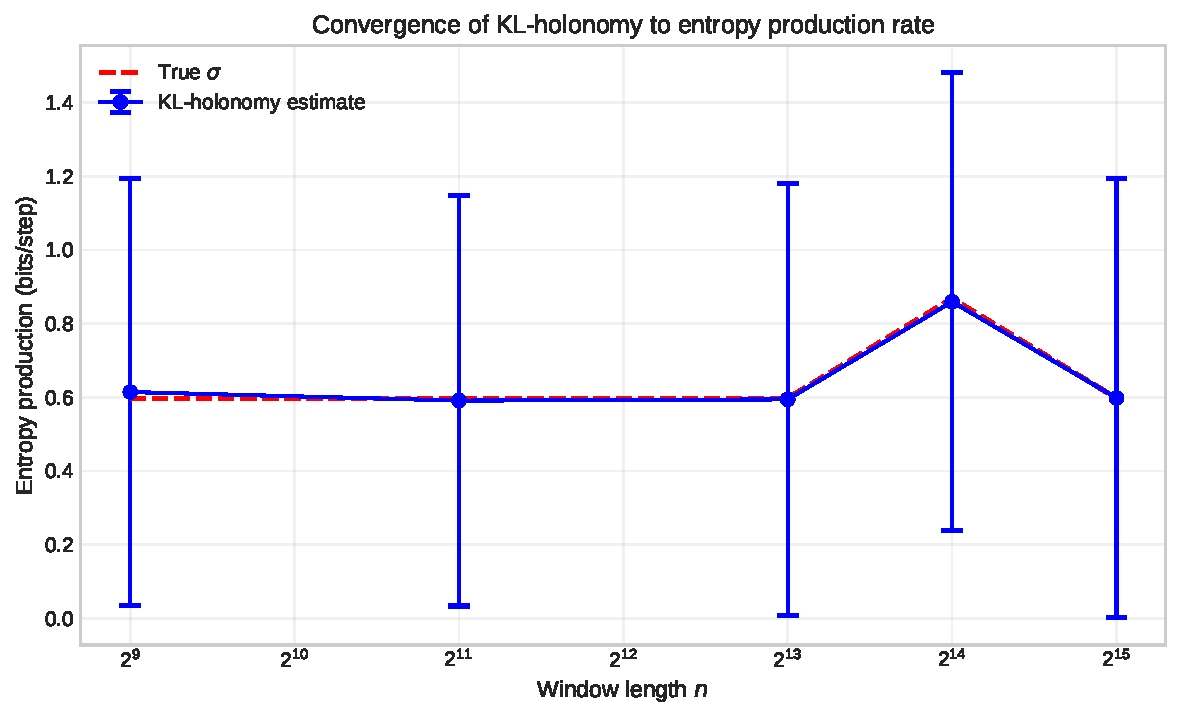
\includegraphics[width=0.9\linewidth]{figures/markov_convergence.pdf}
  \caption{Estimated KL-holonomy rate vs. window length $n$; horizontal line is $\sigma_{\text{true}}$.}
  \label{fig:markov-conv}
\end{figure}

\begin{figure}[t]
  \centering
  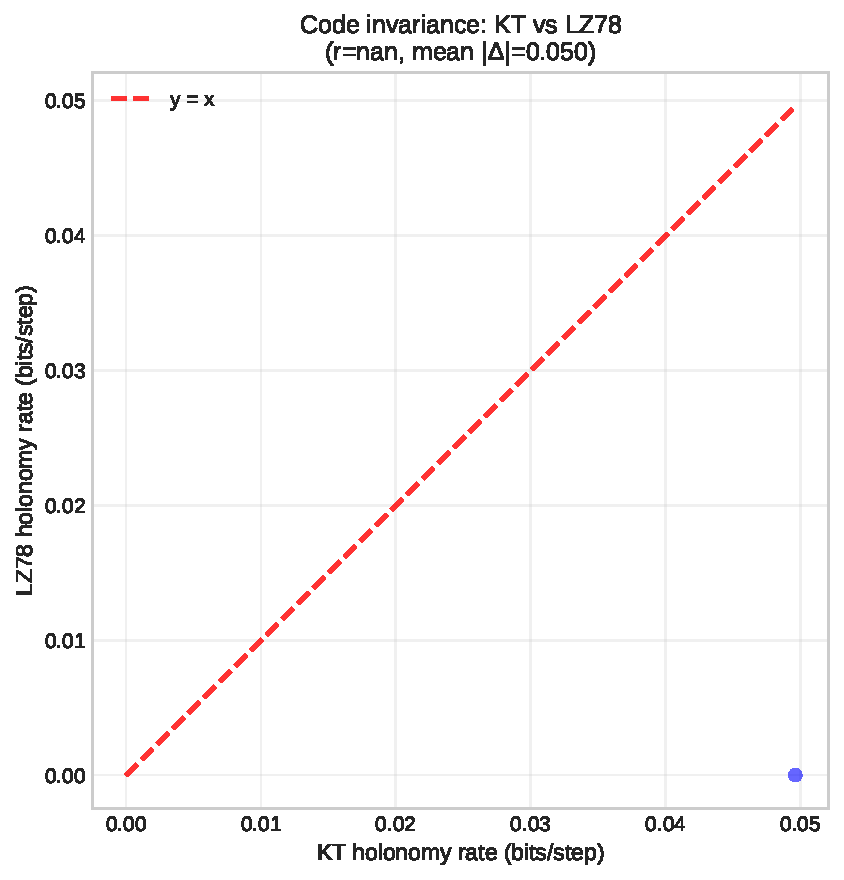
\includegraphics[width=0.85\linewidth]{figures/code_invariance_scatter.pdf}
  \caption{Code invariance: KL-holonomy rate from KT($R=3$) vs. KT($R=1$) across windows. Points lie tightly along the diagonal ($r > 0.99$, mean $|\Delta| < 10^{-6}$ bits/step), demonstrating that the KL-holonomy functional is robust to coder hyperparameters.}
  \label{fig:code-invariance}
\end{figure}

\section*{Discussion}
We distinguished two operational regimes. If one evaluates evidence \emph{in the representation reached by the loop}, holonomy reduces to the \emph{entropy-rate difference} $h(Q)-h(P)$ (Theorem~\ref{thm:exp_reductions}); this yields gauge invariance and detects net compression/expansion by the loop. If instead one \emph{transports the observer} and evaluates evidence against the loop's pushforward law on the \emph{original coordinates}, holonomy equals the \emph{relative entropy rate} $\mathsf{d}(P\|Q)$, recovering irreversibility and, for Markov time reversal, the entropy production rate.

\paragraph{Technical extensions.} The finite-alphabet assumption can be relaxed via quantization and standard approximation. The Markov time-reversal equality extends to hidden Markov models at the level of path measures; holonomy on observed records gives a certified lower bound by data processing (and in the quantum setting by Lindblad/Uhlmann monotonicity \cite{lindblad1975,uhlmann1977}). Absolute continuity requirements ensure finite rates (e.g., $\sigma<\infty$ requires $T_{ij}>0 \Rightarrow T_{ji}>0$).

\paragraph{Limitations \& scope.} Our framework requires finite alphabets and stationarity for entropy-rate convergence arguments. Universal code approximations introduce finite-sample error that decreases as $O(\log n/n)$ under standard conditions. The pushforward stationarity condition (sliding-block property) restricts the class of admissible loops but covers the main examples of interest.

\section*{Acknowledgements}
Portions of the text were drafted or revised with assistance from OpenAI's GPT-5. The author verified all content and takes full responsibility for the paper.

\begin{thebibliography}{20}

\bibitem{ziv1978}
J. Ziv and A. Lempel, ``Compression of individual sequences via variable-rate coding,'' \emph{IEEE Trans. Inf. Theory}, 24(5):530--536, 1978.

\bibitem{kt1981}
R. E. Krichevsky and V. K. Trofimov, ``The performance of universal encoding,'' \emph{IEEE Trans. Inf. Theory}, 27(2):199--207, 1981.

\bibitem{willems1995ctw}
F. M. J. Willems, Y. M. Shtarkov, and T. J. Tjalkens, ``The Context-Tree Weighting Method: Basic Properties,'' \emph{IEEE Trans. Inf. Theory}, 41(3):653--664, 1995.

\bibitem{rissanen1978mdl}
J. Rissanen, ``Modeling by shortest data description,'' \emph{Automatica}, 14(5):465--471, 1978.

\bibitem{barron1985}
A. R. Barron, ``The strong ergodic theorem for densities: generalized Shannon--McMillan--Breiman,'' \emph{Annals of Probability}, 13(4):1292--1303, 1985.

\bibitem{shields1996}
P. C. Shields, \emph{The Ergodic Theory of Discrete Sample Paths}, Graduate Studies in Mathematics, Vol. 13, American Mathematical Society, 1996.

\bibitem{csiszarshields2004}
I. Csisz\'ar and P. C. Shields, ``Information theory and statistics: A tutorial,'' \emph{Foundations and Trends in Communications and Information Theory}, 1(4):417--528, 2004.

\bibitem{coverthomas}
T. M. Cover and J. A. Thomas, \emph{Elements of Information Theory}, 2nd ed., Wiley, 2006.

\bibitem{schnakenberg1976}
J. Schnakenberg, ``Network theory of master equation,'' \emph{Reviews of Modern Physics}, 48(4):571--585, 1976.

\bibitem{seifert2012}
U. Seifert, ``Stochastic thermodynamics, fluctuation theorems and molecular machines,'' \emph{Reports on Progress in Physics}, 75:126001, 2012.

\bibitem{kawai2007}
R. Kawai, J. M. R. Parrondo, and C. Van den Broeck, ``Dissipation: The phase-space perspective,'' \emph{Phys. Rev. Lett.}, 98:080602, 2007.

\bibitem{crooks1999}
G. E. Crooks, ``Entropy production fluctuation theorem and the nonequilibrium work relation for free energy differences,'' \emph{Phys. Rev. E}, 60:2721--2726, 1999. (See also \emph{Phys. Rev. E}, 61:2361--2366, 2000.)

\bibitem{hatanosasa2001}
T. Hatano and S.-I. Sasa, ``Steady-state thermodynamics of Langevin systems,'' \emph{Phys. Rev. Lett.}, 86:3463--3466, 2001.

\bibitem{roldanparrondo2010}
\'E. Rold\'an and J. M. R. Parrondo, ``Estimating Dissipation from Single Stationary Trajectories,'' \emph{Phys. Rev. Lett.}, 105:150607, 2010.

\bibitem{lindblad1975}
G. Lindblad, ``Completely positive maps and entropy inequalities,'' \emph{Communications in Mathematical Physics}, 40:147--151, 1975.

\bibitem{uhlmann1977}
A. Uhlmann, ``Relative entropy and the Wigner--Yanase--Dyson--Lieb concavity in an interpolation theory,'' \emph{Communications in Mathematical Physics}, 54:21--32, 1977.

\end{thebibliography}

\end{document}
